\newpage
\section{Durchführung}
\label{sec:Durchführung}
\subsection{Justierung}
\begin{figure}
  \centering
  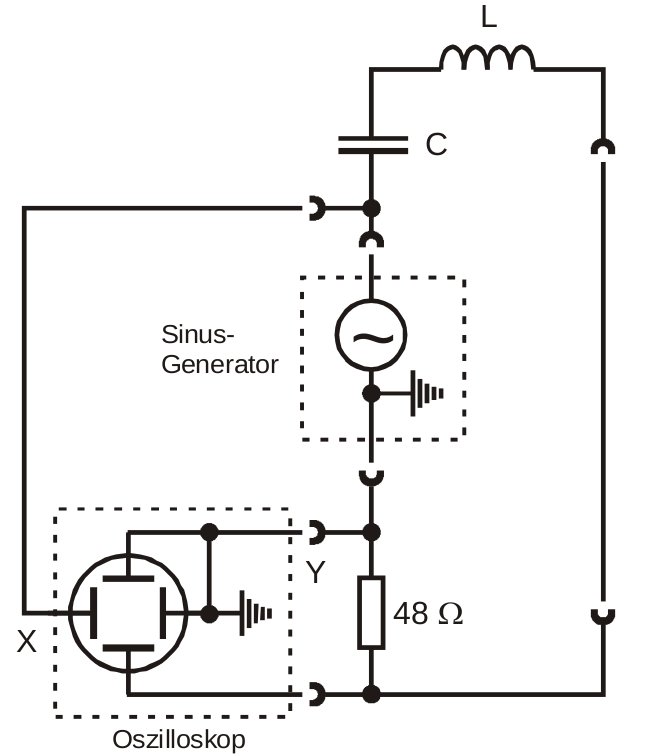
\includegraphics[height= 7cm]{./logos/Abb5.png}
  \caption{Schaltung zur Bestimmung der Resonanzfrequenz eines Schwingkreises\cite{sample}}
  \label{fig:Abb5}
\end{figure}
\FloatBarrier
Zu aller erst wird die Schaltung aus Abbildung \ref{fig:Abb5} realisiert und die Resonanzfrequenz gemessen, die ungefähr beim Strommaximum liegt. Die Feinabstimmung
erfolgt dann durch Lissajous-Figuren, diese bilden eine einfache, gerade Linie im Falle der Resonanz. Anschließend wird  noch eine Schaltung wie in Abb. \ref{fig:Abb5} aufgebaut, jedoch mit dem
abstimmbaren Schwingkreis. In diesem wird die Resonanzfrequenz durch Verstellen der Kapazität auf den gemessenen Wert angeglichen.
\newpage
\subsection{Messprogramm}
\paragraph{Schwingungs-und Schwebungsfrequenz}
\begin{figure}
  \centering
  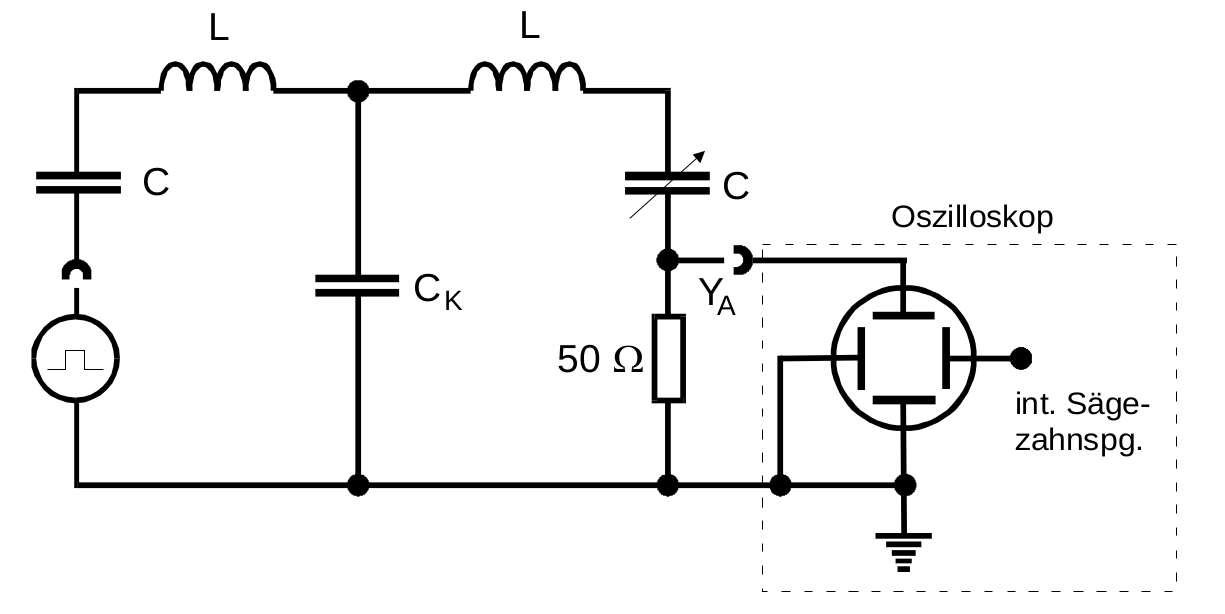
\includegraphics[height = 4.5cm]{./logos/Abb6.png}
  \caption{Schaltung zur Untersuchung von zwei gekoppelten Schwingkreisen\cite{sample}}
  \label{fig:Abb6}
\end{figure}
\FloatBarrier
Nun wird die Schaltung aus Abbildung \ref{fig:Abb6} aufgebaut. Der linke Schwingkreis wird mit einer Rechteckspannung angeregt.
Auf dem Oszilloskop lassen sich dann das Verhältnis von Schwingungs-und Schwebungsfrequenz ablesen. Hierzu werden die Schwingungsmaxima innerhalb der Schwebungsperiode gezählt.
Das Verhältnis der Frequenzen wird für jede Variation von $C_K$ mit $ 2 \leq C_K \leq 12 nF $ gemessen.
\paragraph{Fundamentalschwingungen in Abhängigkeit von $C_K$  bestimmt mit Lissajous-Figuren}
  In diesem Teil des Versuches wird die Rechteckspannung aus Abb. \ref{fig:Abb6} durch ein Sinussignal ersetzt. Nun wird wieder $C_K$ variiert und für
  jeden Wert $ \nu_+$ und $\nu_-$ bestimmt. Die Lissajous-Figuren helfen hier die Frequenzen zu finden bei denen die Phase Null oder $ \pi $ ist.
\paragraph{Fundamentalschwingungen in Abhängigkeit von $C_K$  bestimmt mit der Sweep-Methode}
  Jetzt wird die Sinusspannung mit einem Sweep versehen. Dieser lässt die Sinusspannung in einem einstellbarem Zeitintervall von einer bestimmten Frequenz auf eine andere ansteigen.
  Auf dem Osilloskop kann man dann den Anfang und das Ende des Sweeps beobachten. Bei korrekter Einstellung kann man dort die Resonanzpeaks erkennen. Dabei misst man
  die Zeitintervalle vom Anfang des Sweeps zu jeweils beiden der Resonanzpeaks. Auch bei diesem Teil des Versuches werden alle Werte abhängig vom Koppelkondensators $ C_K$ bestimmt.

  \subsection{Geräte-Daten}
  Schaltung 1:
  \begin{equation*}
    C_1 = 0,8015nF \\
    C_{sp,1} = 0,037nF \\
    L_1 = 32,351mH \\
  \end{equation*}

  Schaltung 2:

  \begin{equation*}
    C_2 = 0,7932nF \\
    C_{sp,2} = 0,028nF \\
    L_2 = 23,954mH \\
  \end{equation*}

  Wobei $C_sp$ die Kapazität der Spule darstellt.
